\section{Improving the Estimation Time}
\label{sec:algorithm}

% \begin{itemize}
% \item For simple degrees we have the flow-algorithm, with $n^2$
%   variables.  I suggest we start with this one.
% \item Even if we consider the naive algorithm with $2^n$ variables, we
%   can optimize it by including only variables needed in the join, plus
%   one extra variable.  (But this seems rather obvious, we should
%   exhaust other contributions first.)
% \item For Berge-acyclic queries we have a much simpler algorithm.
%   Notice that the constraints here need not be acyclic, so this is not
%   subsumed by the flow-algorithm.  This could be a contribution, but
%   it's limited to Berge-acyclic.
% \item We can generalize a little, by considering Berge-decomposition
%   (which we define as a tree decomposition where any two bags share at
%   most one variable).  Then we can combine the flow algorithm with the
%   acyclic algorithm.
% \end{itemize}
% 

\system needs to compute the upper bound in milliseconds in order to
be of use for query optimization.  To achieve this, we start by
applying two simple optimizations to the Basic Algorithm \lpbase in
Sec.~\ref{subsec:basic:algorithm}, which, recall, uses $2^n$ numerical
variables.  (1) for each atom $R_j(V_j)$ of the query, we consolidate
all variables $X_i$ that do not occur anywhere else into a single
variable, and (2) we retain only the \emph{Elemental Basic Shannon
  Inequalities}\footnote{Eq.~\eqref{eq:shannon:submodularity} is
  elemental if it is of the form $h(X_iW)+h(X_jW)\geq h(X_iX_jW)+h(W)$
  where $X_i,X_j$ are single variables and $W$ a set of
  variables;~\eqref{eq:shannon:monotonicity} is elemental if it is of
  the form $h(V)\geq h(V-\set{X_i})$ where $V=\set{X_1, \ldots, X_n}$
  is the set of all variables.}~\cite{Yeung:2008:ITN:1457455} in the
list of constraints, which are known to be complete.  Even with these
optimizations, \lpbase takes 100 ms already for queries with
$n \approx 10$ logical variables $X_1, \ldots, X_n$
(Fig.~\ref{fig:LpBound-estimation-time}).  We describe below two
improvements. \nop{that scale to larger queries.  To simplify the
  presentation, we assume that $Q$ (Eq.~\eqref{eq:cq}) is a full
  conjunctive query.}

\subsection{\lptdb: Berge-Acyclic Queries}

Our first algorithm works under two restrictions: the query needs to
be Berge-acyclic (Sec.~\ref{sec:background}), and all degree
constraints must be full and simple.  These restrictions are actually
quite generous: the JOBjoin, JOBlight, JOBrange, and STATS benchmarks used in Sec.~\ref{sec:experiments}
satisfy them.  Recall that $V= \set{X_1, \ldots, X_n}$ are the
variables of the query $Q$, and $R_1(V_1), \ldots, R_m(V_m)$ are the
atoms of $Q$.  For each variable $X_i$, let $a_i$ denote the number of atoms
that contain it.  We denote by $E_Q$ the following entropic
expression:
%
\begin{align}
  E_Q = & \sum^m_{j=1} h(V_j) - \sum^n_{i=1} (a_i-1) h(X_i) \label{eq:expr:q}
\end{align}
%
The linear program called \lptdb is the following:

\smallskip

\noindent {\bf The Real-valued Variables} are $h(X_1),\ldots,h(X_n)$ and
$h(V_1),\ldots,$ $h(V_m)$. Thus, instead of $2^n$ real-valued variables
$h(U)$, we only have one for each query variable $X_j$, and one for
each set $V_j$ corresponding to an atom $R_j(V_j)$, for a total of
$m+n$.

\smallskip

\noindent {\bf The Objective} is to maximize $E_Q$, under the
following constraints.

\smallskip

\noindent {\bf Statistics Constraints:} all constraints in
Eq.~\eqref{eq:h:p} are included.  This is possible
because the degree sequence is full and simple, and LHS can be written
as $\frac{1}{p}h(U)+h(V|U) = h(UV) - \frac{p-1}{p}h(U)$, where $U$ is
a single variable, and $UV$ is the set of variables of some
relation.

\smallskip

\noindent {\bf Additivity Constraints:} instead of all Shannon
inequalities, we have $1+|V_j|$ constraints for each atom $R_j(V_j)$
(for a total of $m+\sum_j|V_j|$ constraints):
%
\begin{align*}
  h(V_j) \leq & \sum_{i: X_i \in V_j} h(X_i) &\text{and}\ \ \ \ \ h(X_i) \leq  &h(V_j), \forall X_i \in V_j
\end{align*}

\begin{theorem} \label{th:lpbase:eq:lptdb}
  The optimal values of \lpbase and \lptdb are equal.
\end{theorem}

The proof uses techniques from information theory and is included in the supplementary material. 

\begin{example}
  We illustrate \lptdb on the 3-way join query $J_3$ in
  Eq.~\eqref{eq:j3}, and assume for simplicity that the only available
  statistics are the cardinalities (i.e., the $\ell_1$-norm of any
  full degree sequence): $|R|=|S|=|T|=M$, therefore, the AGM bound
  applies: $|J_3|\leq |R|\cdot |T| = M^2$.  The \lptdb is the
  following (where $m \defeq \log M$):
  %
  \begin{align*}
    & \texttt{maximize } E_{J_3}\defeq h(XY)+h(YZ)+h(ZU)-h(Y)-h(Z)\\
    & \text{subject to} \\
    & \ h(XY) \leq m,\ h(YZ) \leq m,\ h(ZU) \leq m\\
    & \ h(X)\leq h(XY),\ h(Y)\leq h(XY),\ h(XY)\leq h(X)+h(Y)\ // \text{for } R(XY)\\
    & \hspace{44mm} \text{similarly for $S(YZ)$ \text{ and } $T(ZU)$}
  \end{align*}
  %
  Notice that we only use 7 real-valued variables: we do not have
  real-valued variables for $h(XYZ)$ or $h(YU)$ etc.  One optimal
  solution is $h^*(X)=\cdots=h^*(U)=m/2$, $h^*(XY)=h^*(YZ)=h^*(ZU)=m$,
  and $E_{J_3}^*=2m$, implying $|J_3|\leq M^2$.  Notice that the
  additivity constraints are important in order to obtain a tight
  bound: if we dropped them, then the linear program admits the
  feasible solution $h^{**}(X)=\cdots=h^{**}(U)=0$,
  $h^{**}(XY)=h^{**}(YZ)=h^{**}(ZU)=m$, and $E_Q^{**}=3m$, leading to
  a weaker bound $|J_3|\leq M^3$.  Thus, the additivity constraints
  are unavoidable.  Statistics beyond cardinalities can easily be
  added, for example, an $\ell_4$ constraint on $\degree_S(Z|Y)$
  becomes
  $\frac{1}{4}h(Y)+h(Z|Y) = h(YZ) - \frac{3}{4}h(Y) \leq \log
  \lp{\degree_S(Z|Y)}_4$.
\end{example}

\lptdb can be adapted to Berge-acyclic queries with group-by as follows. Given a Berge-acyclic query $Q$ with group-by variables $V_0$, we can derive an equivalent Berge-acyclic query $Q'$ by removing from $Q$ the variables that are not in $V_0$ and are not join variables. The full Berge-acyclic query $Q''$, which is obtained from $Q'$ by promoting all variables in $Q'$ to group-by variables, has output size at least that of $Q'$. The quantity returned by \lptdb for $Q''$ is thus a valid upper bound on the size of $Q$.
\begin{example}
    Consider again the Berge-acyclic group-by query StarG in Sec.~\ref{sec:lpbound-groupby-queries}. We rewrite it into 
    \begin{align*}
        \text{StarG}''(X_1,X_2,Z) = R_1(X_1,Z)\wedge R_2(X_2,Z)\wedge S'(Z)
    \end{align*}
    %
    \lptdb maximizes the quantity
    $E_{|\text{StarG}''|} = h(X_1Z) + h(X_2Z) + h(Z) - 2h(Z)$, under
    statistics and additivity constraints.  This yields a better bound
    than~\eqref{eq:sg:bound}, because the statistics constraints
    imply:
    %
    \begin{align*}
      \frac{1}{3}  \log |\dom(S.Z)|  & + \log \lp{\degree_{R_1}(X_1|Z)}_3   + \log \lp{\degree_{R_2}(X_2|Z)}_3 \\
 \geq & \frac{1}{3}h(Z) + \left(\frac{1}{3}h(Z)+h(X_1|Z)\right)+\left(\frac{1}{3}h(Z) + h(X_2|Z)\right)=E_{|\text{StarG}''|}
    \end{align*}
    %
    which leads to the following q-inequality, improving
    over~\eqref{eq:sg:bound}:
    %
    \begin{align*}
      |\text{StarG}| \leq |\text{StarG}''| 
      \leq |\dom(S.Z)|^{1/3}\cdot \lp{\degree_{R_1}(X_1|Z)}_3\cdot\lp{\degree_{R_2}(X_2|Z)}_3
    \end{align*}
% 
%     \begin{align*}
%         E_{|\text{StarG}''|} &= h(X_1Z) + h(X_2Z) + h(Z) - 2h(Z) \\
%         &= \left(\frac{1}{2}h(Z) + h(X_1|Z)\right) + \left(\frac{1}{2}h(Z) + h(X_2|Z)\right) \\
%         &\leq \log \lp{\degree_{R_1}(X_1|Z)}_2 + \log \lp{\degree_{R_2}(X_2|Z)}_2
%     \end{align*}
%     Then, $|\text{StarG}| \leq |\text{StarG}''| \leq \lp{\degree_{R_1}(X_1|Z)}_2\cdot \lp{\degree_{R_2}(X_2|Z)}_2$. For the database in Footnote~5, $\lp{\degree_{R_1}(X_1|Z)}_2 = \lp{\degree_{R_2}(X_2|Z)}_2 $ $= 1$, so \lptdb returns 1, which is the actual output size of StarG.
%     \nop{The bound in Eq.~\eqref{eq:sg:bound} also holds for $\text{StarG}''$, where $|S|$ is replaced by $|S'|$.}
\end{example}

% \lptdb can be more effective when also using statistics constraints on the projected relations.

\nop{, which are norms on non-full degree constraints of the original relations.}

%%%%%%%%%%%%%%%%%%%%%%%%%%%%%%%%  
\subsection{\lpflow: Using Network Flow}
\label{subsec:lpflow}

%%%%%%%%%%%%%%%%%%%%%%%%%%%%%%%%  
\begin{figure}[t]
  \centering
  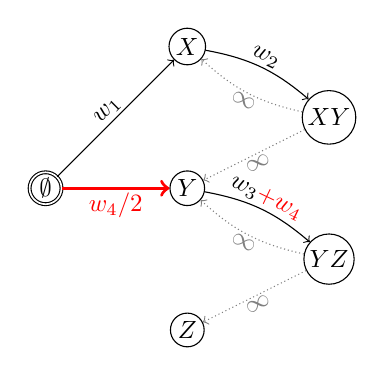
\begin{tikzpicture}[scale = 0.9, every node/.style={transform shape, scale = 1, inner sep = 1.2}]
      \node [draw, circle, double] (phi) at (0,0) {$\emptyset$};
      \node [draw, circle] (X) at (2,+2) {$X$};
      \node [draw, circle] (Y) at (2,0) {$Y$};
      \node [draw, circle] (Z) at (2,-2) {$Z$};
      \node [draw, circle] (XY) at (4,+1) {$XY$};
      \node [draw, circle] (YZ) at (4,-1) {$YZ$};
      \draw (phi) [->] to node[midway, sloped, above]{$w_1$} (X);
      \draw[->, bend left = 15] (X) to node[midway, sloped, above]{$w_2$} (XY);
      \draw[->, gray, densely dotted, bend left = 15] (XY) to node[midway, sloped, below]{$\infty$} (X);
      \draw[->, gray, densely dotted, bend left = 0] (XY) to node[midway, sloped, below]{$\infty$} (Y);
      \draw[->, bend left = 15] (Y) to node[midway, sloped, above]{$w_3${\color{red}${+w_4}$}} (YZ);
      \draw[->, gray, densely dotted, bend left = 15] (YZ) to node[midway, sloped, below]{$\infty$} (Y);
      \draw[->, gray, densely dotted, bend left = 0] (YZ) to node[midway, sloped, below]{$\infty$} (Z);
      \draw (phi) [->, very thick, red] to node[midway, sloped, below=-0.05]{${w_4/2}$} (Y);
      % \draw (XY) [->, gray, densely dotted, bend right = 10] to node[midway, sloped, above]{$\infty$} (phi);
      % \draw (YZ) [->, gray, densely dotted, bend right = -20] to node[midway, sloped, below]{$\infty$} (phi);
    \end{tikzpicture}
  \caption{Example for \lpflow.}
  \label{fig:lpflow}
  \vspace*{-1em}
\end{figure}
%%%%%%%%%%%%%%%%%%%%%%%%%%%%%%%%  

Our second algorithm works for {\em any} conjunctive query (not
necessarily acyclic), and {\em any} constraints (they need to be on
\emph{simple}: recall that we only consider simple degree sequences in
this paper).  Our algorithm consists of a new linear program, \lpflow,
that uses a number of real-valued variables that is quadratic in the
query size: this is much better than the exponential number in
\lpbase, and slightly worse than the linear number in \lptdb. \lpflow
reduces the problem to a collection of network flow problems. It
generalizes the flow-based linear program introduced
in~\cite{DBLP:journals/corr/abs-2211-08381} for the \maxdegree bound
to the general statistics considered by \system.

%
% The basic algorithm of \system from Section~\ref{subsec:basic:algorithm}
% produces a linear program whose size is exponential in $n$, the number of variables in the query.
% This motivates the search for alternative polynomial-time algorithms.
% To that end, we build upon the work in~\cite{DBLP:journals/corr/abs-2211-08381}, which
% studies a special case of our bounds where they only have cardinality and
% maximum-degree constraints. In particular,~\cite{DBLP:journals/corr/abs-2211-08381}
% proposes a polynomial-time algorithm for computing the bound in this special case
% that reduces the problem to a collection of network flow problems.
% We extend this algorithm to handle our more general bounds.
\lpflow is different from both \lpbase and \lptdb. We
describe it only on an example, which illustrates both the original algorithm from~\cite{DBLP:journals/corr/abs-2211-08381}, and our generalization to $\ell_p$-norms. An in-depth account is given in the supplementary material.

\begin{example}
    \label{ex:lpflow}
    Consider the 2-way join $J_2$ in Eq.~\eqref{eq:j2}, along with statistics $|\dom(R.X)|$, $\lp{\degree_R(Y|X)}_\infty$, and
    $\lp{\degree_S(Z|Y)}_\infty$.  Our target is to find coefficients
    $w_1, w_2, w_3$ that make the following q-inequality valid and
    minimize the bound:
\begin{align}
    |J_2| \leq
        |\dom(R.X)|^{w_1} \cdot
        \lp{\degree_R(Y|X)}_\infty^{w_2} \cdot
        \lp{\degree_S(Z|Y)}_\infty^{w_3}
    \label{eq:lpflow:j2}
\end{align}
For that, the following needs to be a valid information inequality:
\begin{align}
    h(XYZ) \leq w_1 h(X) + w_2 h(Y|X) + w_3 h(Z|Y)
    \label{eq:lpflow:j2:ineq}
\end{align}
The key insight from~\cite{DBLP:journals/corr/abs-2211-08381} is that
checking the validity of such inequality (where all degree constraints
are {\em simple}) is equivalent to constructing a flow network
$G=(\nodes,\edges)$, and checking whether each variable $X, Y, Z$ is
independently receiving a maximum flow of at least 1.  In our
example, the flow network $G$ is shown in Fig.~\ref{fig:lpflow}
(ignore the \textbf{\color{red}red} part referring to ${\color{red}w_4}$ for now), where the nodes are the source $\emptyset$, individual variables $\{X\}$, $\{Y\}$, $\{Z\}$,
and sets $\{X, Y\}, \{Y, Z\}$ corresponding to available degree sequences
$\degree_R(Y|X), \degree_S(Z|Y)$.  The edges are of two types:
\begin{itemize}
    \item \textbf{Forward edges} like $X \to XY$ with capacity $w_2$. This represents the term $w_2 h(Y|X)$.
    \item \textbf{\color{gray}Backward edges} like $XY \to X$ with capacity $\infty$. This represents the monotonicity $h(X) \leq h(XY)$.
\end{itemize}



For inequality~\eqref{eq:lpflow:j2:ineq} to be valid,
\begin{itemize}
    \item $X$ needs to receive a flow of at least $1$.  Intuitively,
      this means $w_1 \geq 1$.  
    \item Independently, $Y$ needs to receive a flow of at least
      $1$. Intuitively, there is only one path from the source
      $\emptyset$ to $Y$, which is $\emptyset \to X \to XY \to Y$, and
      this implies that $\min(w_1, w_2, \infty) \geq 1$.  Formally,
      however, we need to setup a standard network flow LP: there is
      one flow variable \nop{for} $f_{a,b}$ for each edge $(a,b)$, with a
      capacity constraint $f_{a,b} \leq w_{a,b}$, and there is one
      flow-preservation constraint for each node (other than source
      and target); e.g., the constraint at node $X$ is
      $f_{\emptyset,X}+f_{XY,X}-f_{X,XY}=0$.
    \item Independently, $Z$ needs to receive a flow of at least
      $1$. Similar to above, this implies that
      $\min(w_1, w_2, \infty, w_3, \infty) \geq 1$, but formally we
      need a separate network flow LP.
\end{itemize}
%
To capture all network flows using a single LP, we simply create three
separate real-valued flow variables for each edge $(a, b)$, namely
$f_{a,b; X}, f_{a,b; Y}, f_{a,b; Z}$.  The \lpflow is shown below 
(ignore the {\bf\color{red} red} text referring to {\color{red}$w_4$} for now): 
  \begin{align}
    \min\quad
        &w_1 \log |\dom(R.X)|+
        w_2 \log \lp{\degree_R(Y|X)}_\infty\label{eq:lpflow:j2:lp:revised}\\
        &\quad +w_3 \log \lp{\degree_S(Z|Y)}_\infty
        {\color{red}+w_4 \log \lp{\degree_S(Z|Y)}_2}\nonumber\\
    \text{s.t.}\quad&w_1, w_2, w_3, {\color{red}{w_4}} \geq 0\nonumber\\
      & (f_{a,b;X})_{(a,b) \in \edges} \text{ form a flow $\emptyset\rightarrow X$ of capacity $\geq 1$}\nonumber\\
      & (f_{a,b;Y})_{(a,b) \in \edges} \text{ form a flow $\emptyset\rightarrow Y$ of capacity $\geq 1$}\nonumber\\
  \end{align}
  \begin{align}
        & (f_{a,b;Z})_{(a,b) \in \edges} \text{ form a flow $\emptyset\rightarrow Z$ of capacity $\geq 1$}\nonumber\\
        & f_{\emptyset,X;*}\leq w_1,\quad
        f_{X,XY;*}\leq w_2,\quad
        f_{Y,YZ;*}\leq w_3 {\color{red}+ w_4},\nonumber\\
        &{\color{red}f_{\emptyset,Y;*}\leq w_4/2}\nonumber
  \end{align}

There are $3n\sum_j |V_j|$ total variables, because the network has
$2\sum_j|V_j|$ edges, and for each edge $(a,b)$ we need to create one
capacity variable $w_{a,b}$, and $n$ real-valued variables:
$f_{a,b;X_i}$, $i=1,n$.


% 
% And now minimizing the bound from Eq.~\eqref{eq:lpflow:j2} corresponds to solving the
% linear program in Fig.
% 
% 
% \begin{align}
%     \min\quad
%         &w_1 \log |\dom(R.X)|+
%         w_2 \log \lp{\degree_R(Y|X)}_\infty\label{eq:lpflow:j2:lp}\\
%         &\quad +w_3 \log \lp{\degree_S(Z|Y)}_\infty\nonumber\\
%     \text{s.t.}\quad
%         &w_1 \geq 1,\quad
%         \min(w_1, w_2) \geq 1,\quad
%         \min(w_1, w_2, w_3) \geq 1\nonumber\\
%         &w_1, w_2, w_3 \geq 0\nonumber
% \end{align}
% The flow network is always polynomial-sized and so is the above linear program.

We next outline how to generalize the above algorithm to handle bounds
on arbitrary $\ell_p$-norms of degree sequences.  Continuing with the
above example, suppose that we are additionally given  $\lp{\degree_S(Z|Y)}_2$.  The RHS of the
q-inequality~\eqref{eq:lpflow:j2} now has an additional factor of
$\lp{\degree_S(Z|Y)}_2^{w_4}$ where $w_4$ is a new coefficient.
Similarly, the RHS of inequality~\eqref{eq:lpflow:j2:ineq} now has two
additional terms $+\frac{w_4}{2}h(Y) + w_4 h(Z|Y)$.  Accordingly, the
flow network from Fig.~\ref{fig:lpflow} is extended with extra
edges, depicted in \textbf{\color{red}red}.  In particular, we
have an extra edge from $\emptyset$ to $Y$ with capacity $w_4/2$, and
an extra edge from $Y$ to $YZ$ adding a capacity of $w_4$, on top of
the existing capacity of $w_3$.  These extra edges lead to new paths
that can be used to send flow to $Y$ and $Z$.  As a result, the
objective function of the above linear program is
extended with the red term.  The capacity constraints on the red
edges also change: They become $f_{\emptyset, Y; X} \leq w_4/2$,
$f_{\emptyset, Y; Y} \leq w_4/2$, $f_{\emptyset, Y; Z} \leq w_4/2$,
and similarly $f_{Y,YZ;X} \leq w_3+w_4$ etc.
% \begin{align}
%     \max\quad
%         &w_1 \log |\dom(R.X)|+
%         w_2 \log \lp{\degree_R(Y|X)}_\infty\label{eq:lpflow:j2:lp:revised}\\
%         &\quad +w_3 \log \lp{\degree_S(Z|Y)}_\infty
%         {\color{red}+w_4 \log \lp{\degree_S(Z|Y)}_2}\nonumber\\
%     \text{s.t.}\quad
%         &w_1 \geq 1,\quad
%         \min(w_1, w_2) {\color{red}+ \frac{w_4}{2}} \geq 1,\nonumber\\
%         &{\color{red}\min\left(\min(w_1, w_2) + \frac{w_4}{2}, w_3 + w_4\right) \geq 1}\nonumber\\
%         &w_1, w_2, w_3, {\color{red}w_4} \geq 0\nonumber
% \end{align}
\end{example}
The above bound can be straightforwardly generalized to handle \groupby by only considering flows $f_{a, b; X_i}$ where $X_i$ is a \groupby.

We prove the following theorem in the supplementary material.
\begin{theorem} \label{th:lpbase:eq:lpflow}
    The optimal values of \lpbase and \lpflow are equal.
  \end{theorem}


\subsection{Putting them Together}

Given a query $Q$, \system checks if $Q$ is Berge-acyclic and if all
statistics are full (they are always simple), and, in that case it
uses \lptdb to compute the bound, since its size is only linear in the
size of $Q$ and the statistics.  Otherwise, it uses \lpflow, whose
size is quadratic in the size of the query.  
